\chapter{}
\section{Crystal momentum}
Remember band diagrams derived in previous section \ref{sec:nearly_free_e_approx}. To introduce the crystal momentum, let's first look at
\begin{align}
	&\left\{
	\begin{array}{lr}
		\hat{H} = \frac{\hat{p}}{2m} = -\frac{\hbar^2}{2m}\nabla^2 \qquad\qquad \text{with: } \hat{\vec{p}} = -n\hbar\vec{\nabla}\\
		\hat{H}\psi_{\vec{k}}(\vec{r}) = E \psi_{\vec{k}}(\vec{r}) \\
		\psi_{\vec{k}} = \frac{1}{\sqrt{V}}e^{i\vec{k}\cdot\vec{r}}
	\end{array}\right\\
	&[\hat{H}, \hat{\vec{p}}] = 0\\
	\text{using de Brogli:}\qquad & \vec{p} = \hbar\vec{k} \label{eqn:brogli_relation}\\
	\text{we get:}\qquad &\hat{\vec{p}}\psi_{\vec{k}}(\vec{r}) = \hbar\vec{k}\psi_{\vec{k}}(\vec{r})
\end{align}
Bloch electrons: $\hat{H} = p^2/2m + V(\vec{r})$, with $\hat{\vec{p}} = -i\hbar\vec{\nabla}$.
Then now it is clear that these operators $[\hat{H}, \hat{\vec{p}}] \neq 0$
Then we can derive the following:
\begin{align}
	\hat{H}\psi_{n, \vec{k}}(\vec{r}) &= E_n(\vec{k})\psi_{n, \vec{k}}(\vec{r})\\
	\psi_{n, \vec{k}}(\vec{r}) &= u_{n, \vec{k}}(\vec{r})e^{i\vec{k}\cdot\vec{r}} \label{eqn:psi_bloch}\\
	\hat{\vec{p}}\psi_{n, \vec{k}}(\vec{r}) &= -i\hbar\vec{\nabla}\left[u_{n, \vec{k}}(\vec{r})e^{i\vec{k}\cdot\vec{r}}\right] \qquad \text{using: \ref{eqn:brogli_relation} and \ref{eqn:psi_bloch}}\\
\end{align}
How do we interpret the $\vec{k}$? Let's define crystal momentum as follows:
\begin{equation}
	\vec{P} = \hbar\vec{k}
\end{equation}
\nt{Don't confuse $\vec{P}$ with $\vec{p}$. For a Bloch electron we cannot say that $\vec{p} = \hbar\vec{k}$.}

Because real space is infinite, we need some boundary condiditions to confine our space.
\section{Boundary condition}
There are two possiblities to impose boundary conditions:
\begin{itemize}
	\setlength\itemsep{0pt}
	\item Dirichlet boundary conditions
	\item Born-von Kerman (periodic) boundary conditions
\end{itemize}
We will use periodic boundary conditions to show how energy bands are formed in an atomic crystal. The reason we use periodic boundary conditions is that this makes math easier, you do get the same result when using Dirichlet boundary conditions.
\ex{1D boundary condition}{
	For the function $\psi(x) = \psi(x + L)$, with $L$ the crystal length. 
	\begin{center}
		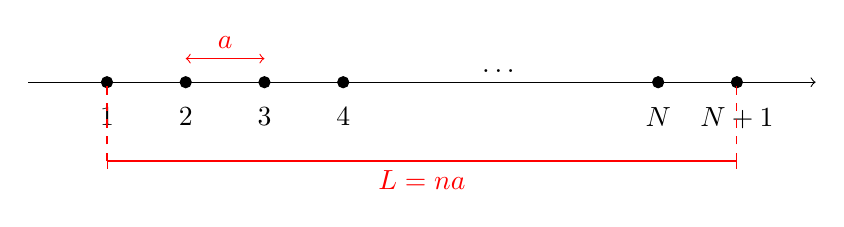
\begin{tikzpicture}
			\draw[->, black]	(0, 0) to (10, 0);

			\filldraw[black]	(1, 0) node[below=2mm]{$1$} circle (2pt)
								(2, 0) node[below=2mm]{$2$} circle (2pt)
								(3, 0) node[below=2mm]{$3$} circle (2pt)
								(4, 0) node[below=2mm]{$4$} circle (2pt)
								(8, 0) node[below=2mm]{$N$} circle (2pt)
								(9, 0) node[below=2mm]{$N+1$} circle (2pt);

			\draw[black]		(6, 0) node[above]{\dots};

			\draw[<->, red]		(2, 0.3) to node[above]{$a$} (3, 0.3);
			\draw[|-|, red]		(1, -1)	to node[below]{$L = na$} (9, -1);

			\draw[dashed, red]	(1, -1) to (1, 0)
								(9, -1) to (9, 0);
		\end{tikzpicture}
	\end{center}
	We can use some properties of the bloch functions, now we can deduce the following:
	\begin{align}
		\psi(x + L) &= e^{ikL}\psi(x) = \psi(x)\\
		&\Rightarrow kNa = 2\pi n \\
		&\Rightarrow k = \frac{2\pi}{L}n
	\end{align}
	We see that the continious $k$ value has become discrete, therefore we get the following figure. As we might expect, for a bigger lattice, we get a more continious spectrum (because $\Delta k$ becomes smaller).
	\begin{center}
		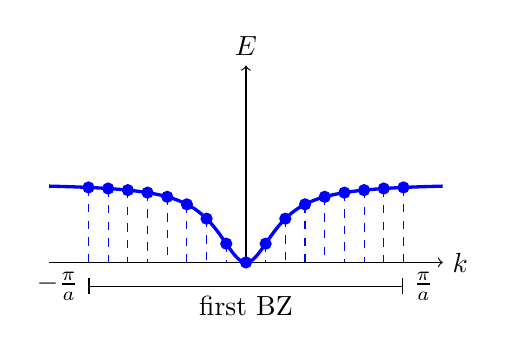
\begin{tikzpicture}[domain=-2.5:2.5]
			\draw[->] (-2.5,0) -- (2.5,0) node[right] {$k$};
			\draw[->] (0,0) -- (0,2.5) node[above] {$E$};

			\draw[blue, very thick] plot[samples=200] (\x, {1 - 1/(1 + 5*\x*\x)});

			\foreach \x in {-8,...,8} {
				\filldraw[blue]	({\x / 4}, {1 - 1/(1 + 5*\x*\x / 16)}) circle (2pt);
				\draw[dashed, blue]	({\x / 4}, {1 - 1/(1 + 5*\x*\x / 16)}) to ({\x / 4}, 0);
			}

			\draw	(-2, -0.3)	node[left]{$-\frac{\pi}{a}$};
			\draw	(2, -0.3)	node[right]{$\frac{\pi}{a}$};

			\draw[|-|]	(-2, -0.3) to node[below]{first BZ} (2, -0.3);
		\end{tikzpicture}
	\end{center}
	How many lattice points do we have in our first BZ?
	\begin{equation}
		\frac{\frac{2\pi}{a}}{\Delta k} = \frac{\frac{2\pi}{a}}{\frac{2\pi}{Na}} = N = \text{number of unit cells that build the crystal}
	\end{equation}
}
Can we come to the same conclusion in 3D?
\ex{3D boundary condition}{
	The full crystal is defined by $L_1$, $L_2$, $L_3$. For these values, we can say that:
	\begin{align}
		\left\{
		\begin{array}{lr}
		\vec{L_1} = N_1\vec{a}_1\\
		\vec{L_2} = N_2\vec{a}_2\\
		\vec{L_3} = N_3\vec{a}_3
		\end{array}
		\right
	\end{align}
	We can do the same as we did in the 1D example:
	\begin{align}
		\psi(\vec{r} + \vec{L}_j) &= \psi(\vec{r})\\
		&= \psi(\vec{r} + N_j\vec{a}_j)\\
		\text{Using Bloch}\qquad &\Rightarrow \psi(\vec{r}) = e^{i\vec{k}\cdotN_j\vec{a}_j}\psi(\vec{r})\\
		&\Rightarrow \vec{k} = 2\pi n \cdot (N_j \vec{a}_j)^{-1} \text{with } n \in \bbZ\\
		&\Rightarrow \vec{k} = \frac{n_1}{N_1}\vec{b}_1 + \frac{n_2}{N_2}\vec{b}_2 + \frac{n_3}{N_3}\vec{b}_3
	\end{align}

	$\vec{b}_i$ are primitive reciprocal lattice vectors.

	Now we look at the elemental volume of the unit cell:
	\begin{align}
		\Delta \vec{k} = \Delta k^3 &= \frac{\vec{b}_1}{N_1}\cdot\left(\frac{\vec{b}_2}{N_2} \cross \frac{\vec{b}_3}{N_3}\right)\\
		&= \frac{1}{N}\vec{b}_1\cdot\left(\vec{b}_2 \cross \vec{b}_3\right)
	\end{align}
	Where N is the number of unit cells that build the crystal.
}
We do get the same results, and this has some consequences when we look at the atomic picture of energy bands and how boundary conditions affect them.
\begin{enumerate}
	\setlength\itemsep{0pt}
	\item Even number of electrons in a full shell per unit cell. We get $2N =$ amount of electrons. This gives a semiconductor.
	\item Odd number of electrons in apartially filled shell per unit cell. Because there are still states free in the valence band, gives this a metal.
\end{enumerate}
\nt{This does not mean that a $2N$ amount of electrons gives a semiconductor. Band overlap can still give a metal!}
We now link this concept to real atoms.

\subsection{Energy bands for the atomic picture}
Say, we have $N$ atoms. Then, for each atom we have the states in figure \ref{fig:state_one_atom}. Now suppose we have them far apart and bring them closer, then we get figure \ref{fig:bands_crystal_fictiveatoms}. For a semiconductor, we see a bandgap $E_g$ at $d = a$, this is highlighted in red.
\begin{figure}[h]
	\centering
	\begin{tikzpicture}
		\draw[-, black, very thick]	(0, 0) to (3, 0) node[right]{1s}
									(0, 2) to (3, 2) node[right]{2s};

		\draw[->, black]	(-0.5, -0.5) to (-0.5, 2.5) node[right]{$E$};
	\end{tikzpicture}
	\caption{The energy state for a fictive single atom}
	\label{fig:state_one_atom}
\end{figure}
\begin{figure}[h]
	\centering
	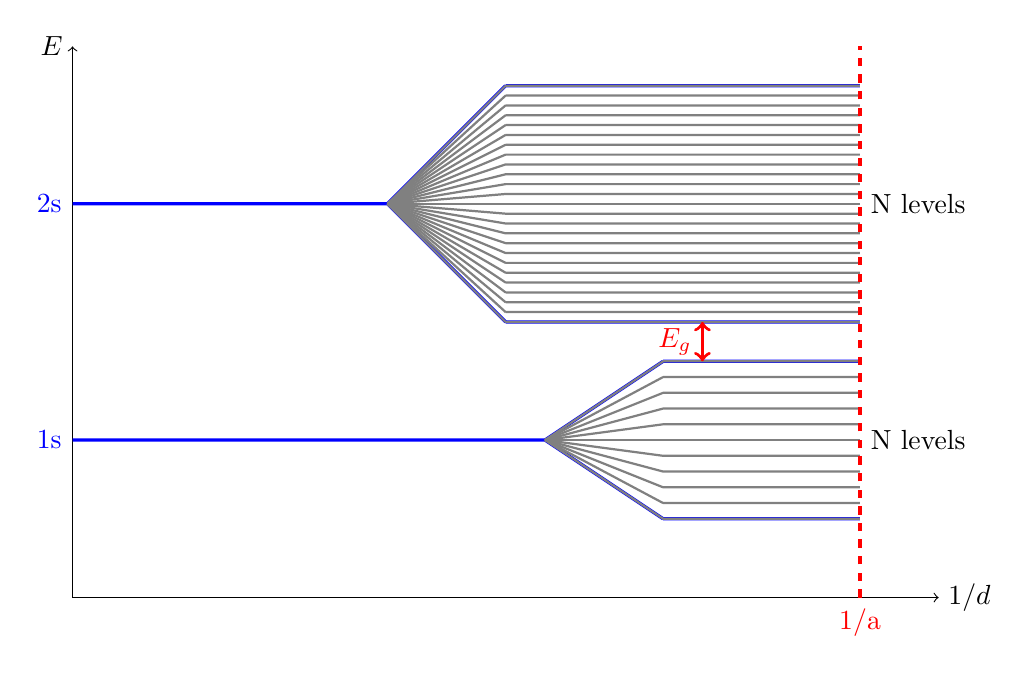
\begin{tikzpicture}
		\draw[->, black]	(0, 0) to (0, 7) node[left]{$E$};
		\draw[->, black]	(0, 0) to (11, 0) node[right]{$1/d$};

		\draw[-, blue, very thick]		(0, 2) node[left]{1s} to (6, 2)
							(6, 2) to (7.5, 3)
							(6, 2) to (7.5, 1)
							(7.5, 3) to (10, 3)
							(7.5, 1) to (10, 1);

		\draw[-, blue, very thick]		(0, 5) node[left]{2s} to (4, 5)
							(4, 5) to (5.5, 6.5)
							(4, 5) to (5.5, 3.5)
							(5.5, 6.5) to (10, 6.5)
							(5.5, 3.5) to (10, 3.5);

		\foreach \y in {28, ..., 52} {
			\draw[-, gray, thick]	(5.5, {\y/8}) to (10, {\y/8})
									(4, 5) to (5.5, {\y/8});
		}

		\foreach \y in {5, ..., 15} {
			\draw[-, gray, thick]	(7.5, {\y/5}) to (10, {\y/5})
									(6, 2) to (7.5, {\y/5});
		}

		\draw[red, very thick]	(10, 0) node[below]{1/a};
		\draw[dashed, red, very thick]	(10, 0) to (10, 7);

		\draw[black, very thick]	(10, 5) node[right]{N levels};
		\draw[black, very thick]	(10, 2) node[right]{N levels};

		\draw[<->, red, very thick]	(8, 3) to node[left]{$E_g$} (8, 3.5);
	\end{tikzpicture}
	\caption{Energy band diagram for fictive crystal of N atoms}
	\label{fig:bands_crystal_fictiveatoms}
\end{figure}
This just shows how the bands are for the atoms, nothig can be said about momentum, \dots. What we notice from the picture, too is:
\begin{itemize}
	 \setlength\itemsep{0pt}
	\item 2s orbital starts to split sooner, because 2s oribitals overlap more as they are furhter away from the nucleus.
	\item We see a smaller band splitting at 1s.
\end{itemize}
We will now look at some other atoms.
\newpage
\ex{Lithium (Li)}{
	For 1 Li atom we have what can be seen in following figure:
	\begin{center}
		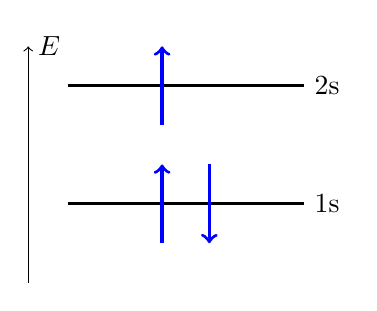
\begin{tikzpicture}
			\draw[-, black, very thick]	(0, 0.5) to (3, 0.5) node[right]{1s}
										(0, 2) to (3, 2) node[right]{2s};

			\draw[->, blue, very thick]	(1.2, 0) to (1.2, 1);
			\draw[->, blue, very thick]	(1.8, 1) to (1.8, 0);
			\draw[->, blue, very thick]	(1.2, 1.5) to (1.2, 2.5);

			\draw[->, black]	(-0.5, -0.5) to (-0.5, 2.5) node[right]{$E$};
		\end{tikzpicture}
	\end{center}

	For $Li_2$ we get:
	\begin{center}
		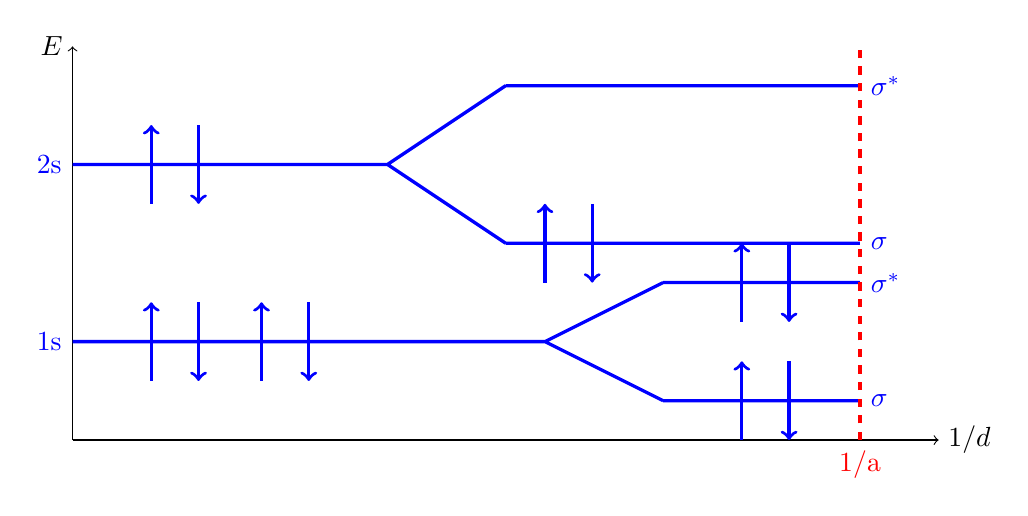
\begin{tikzpicture}
			\draw[->, black]	(0, 0) to (0, 5) node[left]{$E$};
			\draw[->, black]	(0, 0) to (11, 0) node[right]{$1/d$};

			\draw[-, blue, very thick]		(0, 1.25) node[left]{1s} to (6, 1.25)
								(6, 1.25) to (7.5, 2)
								(6, 1.25) to (7.5, 0.5)
								(7.5, 2) to (10, 2) node[right]{$\sigma^{*}$}
								(7.5, 0.5) to (10, 0.5) node[right]{$\sigma$};

			\draw[-, blue, very thick]		(0, 3.5) node[left]{2s} to (4, 3.5)
								(4, 3.5) to (5.5, 4.5)
								(4, 3.5) to (5.5, 2.5)
								(5.5, 4.5) to (10, 4.5) node[right]{$\sigma^{*}$}
								(5.5, 2.5) to (10, 2.5) node[right]{$\sigma$};

			\draw[red, very thick]	(10, 0) node[below]{1/a};
			\draw[dashed, red, very thick]	(10, 0) to (10, 5);

			\draw[->, blue, very thick]	(1, 0.75) to (1, 1.75);
			\draw[->, blue, very thick]	(1.6, 1.75) to (1.6, 0.75);
			\draw[->, blue, very thick]	(2.4, 0.75) to (2.4, 1.75);
			\draw[->, blue, very thick]	(3, 1.75) to (3, 0.75);
			\draw[->, blue, very thick]	(1, 3) to (1, 4);
			\draw[->, blue, very thick]	(1.6, 4) to (1.6, 3);
			\draw[->, blue, very thick]	(8.5, 0) to (8.5, 1);
			\draw[->, blue, very thick]	(9.1, 1) to (9.1, 0);
			\draw[->, blue, very thick]	(8.5, 1.5) to (8.5, 2.5);
			\draw[->, blue, very thick]	(9.1, 2.5) to (9.1, 1.5);
			\draw[->, blue, very thick]	(6, 2) to (6, 3);
			\draw[->, blue, very thick]	(6.6, 3) to (6.6, 2);
		\end{tikzpicture}
	\end{center}

	For a crystal $Li_N$ we get:
	\begin{center}
		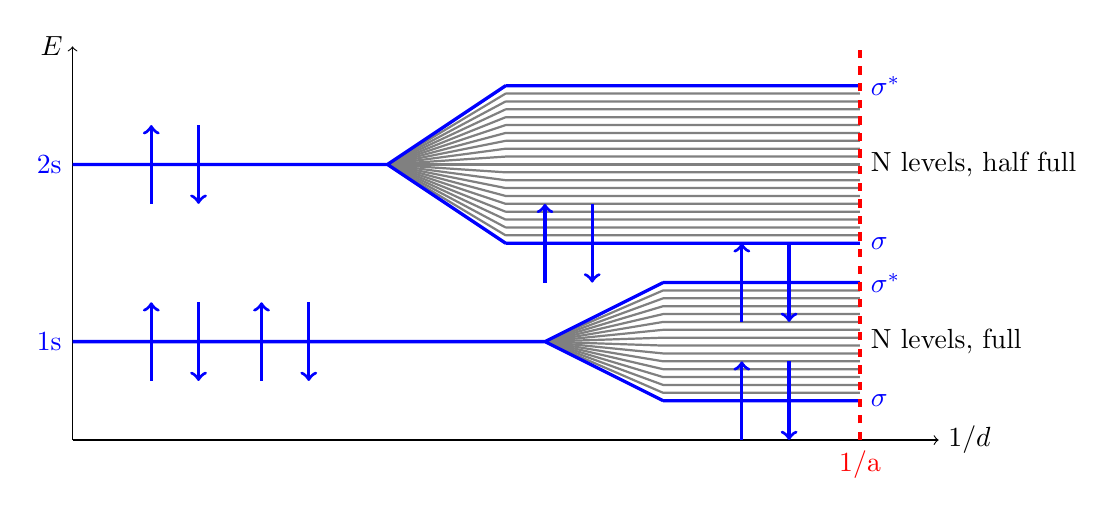
\begin{tikzpicture}
			\draw[->, black]	(0, 0) to (0, 5) node[left]{$E$};
			\draw[->, black]	(0, 0) to (11, 0) node[right]{$1/d$};

			\foreach \y in {5, ..., 20} {
				\draw[-, gray, thick]	(7.5, {\y/10}) to (10, {\y/10})
										(6, 1.25) to (7.5, {\y/10});
			}

			\draw[-, blue, very thick]		(0, 1.25) node[left]{1s} to (6, 1.25)
								(6, 1.25) to (7.5, 2)
								(6, 1.25) to (7.5, 0.5)
								(7.5, 2) to (10, 2) node[right]{$\sigma^{*}$}
								(7.5, 0.5) to (10, 0.5) node[right]{$\sigma$};

			\foreach \y in {25, ..., 45} {
				\draw[-, gray, thick]	(5.5, {\y/10}) to (10, {\y/10})
										(4, 3.5) to (5.5, {\y/10});
			}

			\draw[-, blue, very thick]		(0, 3.5) node[left]{2s} to (4, 3.5)
								(4, 3.5) to (5.5, 4.5)
								(4, 3.5) to (5.5, 2.5)
								(5.5, 4.5) to (10, 4.5) node[right]{$\sigma^{*}$}
								(5.5, 2.5) to (10, 2.5) node[right]{$\sigma$};

			\draw[red, very thick]	(10, 0) node[below]{1/a};
			\draw[dashed, red, very thick]	(10, 0) to (10, 5);

			\draw[->, blue, very thick]	(1, 0.75) to (1, 1.75);
			\draw[->, blue, very thick]	(1.6, 1.75) to (1.6, 0.75);
			\draw[->, blue, very thick]	(2.4, 0.75) to (2.4, 1.75);
			\draw[->, blue, very thick]	(3, 1.75) to (3, 0.75);
			\draw[->, blue, very thick]	(1, 3) to (1, 4);
			\draw[->, blue, very thick]	(1.6, 4) to (1.6, 3);
			\draw[->, blue, very thick]	(8.5, 0) to (8.5, 1);
			\draw[->, blue, very thick]	(9.1, 1) to (9.1, 0);
			\draw[->, blue, very thick]	(8.5, 1.5) to (8.5, 2.5);
			\draw[->, blue, very thick]	(9.1, 2.5) to (9.1, 1.5);
			\draw[->, blue, very thick]	(6, 2) to (6, 3);
			\draw[->, blue, very thick]	(6.6, 3) to (6.6, 2);

			\draw[black, very thick]	(10, 3.5) node[right]{N levels, half full};
			\draw[black, very thick]	(10, 1.25) node[right]{N levels, full};
		\end{tikzpicture}
	\end{center}
}
\ex{Silicium (Si)}{
	Si has following configuration: $1s^2\,2s^2\,2p^6\,3s^2\,3p^2$. This translates in the following band structure:
	\begin{center}
		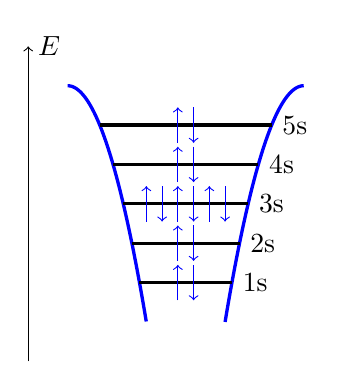
\begin{tikzpicture}
			\draw[blue, very thick] plot[samples=200, domain=0:1] (\x, {-3*\x*\x + 3});
			\draw[blue, very thick] plot[samples=200, domain=2:3] (\x, {-3*(\x - 3)*(\x - 3) + 3});

			\foreach \y in {1, ..., 5} {
				\draw[-, black, very thick]	({ ((\y/2 - 3)/-3)^(1/2) }, \y/2) to ( {-((\y/2 - 3)/-3)^(1/2) + 3}, \y/2) node[right]{\text{\y}s};

				\draw[->, blue]	(1.4, \y/2 - 0.225) to (1.4, {\y/2 + 0.225});
				\draw[->, blue]	(1.6, {\y/2 + 0.225}) to (1.6, \y/2 - 0.225);
			}

			\draw[->, blue]	({1.4 - 0.4}, {3/2 - 0.225}) to ({1.4 - 0.4}, {3/2 + 0.225});
			\draw[->, blue]	({1.6 - 0.4}, {3/2 + 0.225}) to ({1.6 - 0.4}, {3/2 - 0.225});

			\draw[->, blue]	({1.4 + 0.4}, {3/2 - 0.225}) to ({1.4 + 0.4}, {3/2 + 0.225});
			\draw[->, blue]	({1.6 + 0.4}, {3/2 + 0.225}) to ({1.6 + 0.4}, {3/2 - 0.225});

			\draw[->, black]	(-0.5, -0.5) to (-0.5, 3.5) node[right]{$E$};
		\end{tikzpicture}
	\end{center}
	For a Si crystal we have $N$ unit cells. Si cyrstals have a diamond structure with 2 atoms per unit cell. The according band diagram is:
	\begin{center}
		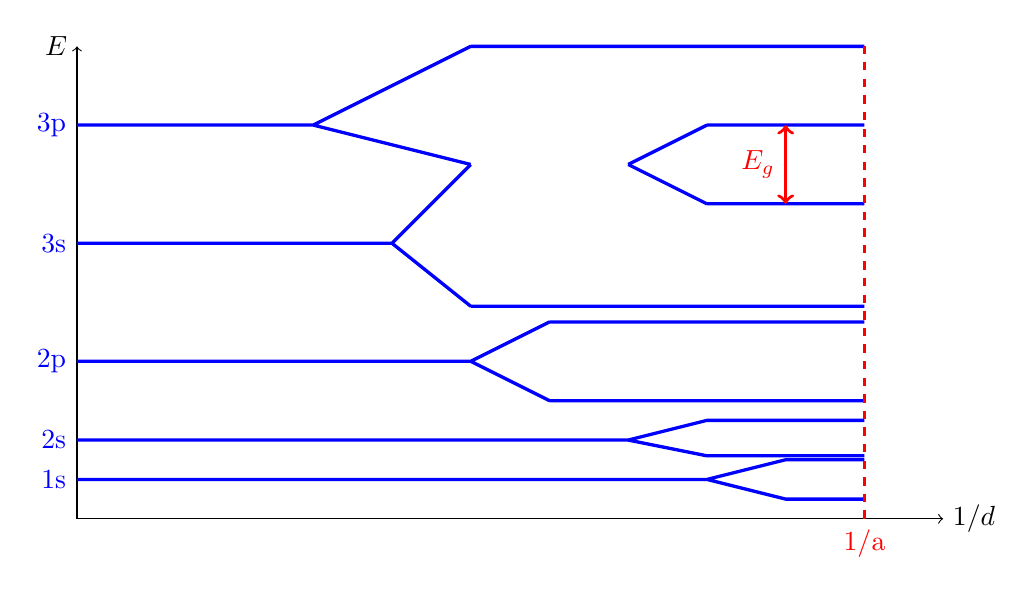
\begin{tikzpicture}
			\draw[->, black]	(0, 0) to (0, 6) node[left]{$E$};
			\draw[->, black]	(0, 0) to (11, 0) node[right]{$1/d$};

			\draw[-, blue, very thick]		(0, 0.5) node[left]{1s} to (8, 0.5)
											(8, 0.5) to (9, 0.25)
											(8, 0.5) to (9, 0.75)
											(9, 0.25) to (10, 0.25)
											(9, 0.75) to (10, 0.75);

			\draw[-, blue, very thick]		(0, 1) node[left]{2s} to (7, 1)
											(7, 1) to (8, 1.25)
											(7, 1) to (8, 0.8)
											(8, 1.25) to (10, 1.25)
											(8, 0.8) to (10, 0.8);

			\draw[-, blue, very thick]		(0, 2) node[left]{2p} to (5, 2)
											(5, 2) to (6, 2.5)
											(5, 2) to (6, 1.5)
											(6, 2.5) to (10, 2.5)
											(6, 1.5) to (10, 1.5);

			\draw[-, blue, very thick]		(0, 3.5) node[left]{3s} to (4, 3.5)
											(4, 3.5) to (5, 4.5)
											(4, 3.5) to (5, 2.7)
											(5, 2.7) to (10, 2.7)
											(7, 4.5) to (8, 4)
											(8, 4) to (10, 4);

			\draw[-, blue, very thick]		(0, 5) node[left]{3p} to (3, 5)
											(3, 5) to (5, 6)
											(3, 5) to (5, 4.5)
											(5, 6) to (10, 6)
											(7, 4.5) to (8, 5)
											(8, 5) to (10, 5);

			\draw[red, very thick]	(10, 0) node[below]{1/a};
			\draw[dashed, red, very thick]	(10, 0) to (10, 6);

			\draw[<->, red, very thick]	(9, 4) to node[left]{$E_g$} (9, 5);
		\end{tikzpicture}
	\end{center}
	If we now consider that each each unit cell has 2 atoms in a silicon lattice, we get the following states for the energy diagram (simplified):
	\begin{center}
		\begin{tikzpicture}
			\draw[->, black]	(0, 0) to (0, 6) node[left]{$E$};
			\draw[->, black]	(0, 0) to (11, 0) node[right]{$1/d$};

			\foreach \y in {2.5, ..., 7.5} {
				\draw[-, gray, thick]	(9, {\y/10}) to (10, {\y/10})
										(8, 0.5) to (9, {\y/10});
			}

			\foreach \y in {8, ..., 12.5} {
				\draw[-, gray, thick]	(8, {\y/10}) to (10, {\y/10})
										(7, 1) to (8, {\y/10});
			}

			\foreach \y in {15, ..., 25} {
				\draw[-, gray, thick]	(6, {\y/10}) to (10, {\y/10})
										(5, 2) to (6, {\y/10});
			}

			\foreach \y in {27, ..., 45} {
				\draw[-, gray, thick]	(5, {\y/10}) to (7, {\y/10})
										(4, 3.5) to (5, {\y/10})
										(7, {\y/10}) to (8, {\y/15 + 0.9})
										(8, {\y/15 + 0.9}) to (10, {\y/15 + 0.9});
			}

			\foreach \y in {45, ..., 60} {
				\draw[-, gray, thick]	(5, {\y/10}) to (7, {\y/10})
										(3, 5) to (5, {\y/10})
										(7, {\y/10}) to (8, {\y/16 + 2.2})
										(8, {\y/16 + 2.2}) to (10, {\y/16 + 2.2});
			}

			\draw[-, blue, very thick]		(0, 0.5) node[left]{1s} to (8, 0.5)
											(8, 0.5) to (9, 0.25)
											(8, 0.5) to (9, 0.75)
											(9, 0.25) to (10, 0.25)
											(9, 0.75) to (10, 0.75);

			\draw[-, blue, very thick]		(0, 1) node[left]{2s} to (7, 1)
											(7, 1) to (8, 1.25)
											(7, 1) to (8, 0.8)
											(8, 1.25) to (10, 1.25)
											(8, 0.8) to (10, 0.8);

			\draw[-, blue, very thick]		(0, 2) node[left]{2p} to (5, 2)
											(5, 2) to (6, 2.5)
											(5, 2) to (6, 1.5)
											(6, 2.5) to (10, 2.5)
											(6, 1.5) to (10, 1.5);

			\draw[-, blue, very thick]		(0, 3.5) node[left]{3s} to (4, 3.5)
											(4, 3.5) to (5, 4.5)
											(4, 3.5) to (5, 2.7)
											(5, 2.7) to (10, 2.7)
											(7, 4.5) to (8, 4)
											(8, 4) to (10, 4);

			\draw[-, blue, very thick]		(0, 5) node[left]{3p} to (3, 5)
											(3, 5) to (5, 6)
											(3, 5) to (5, 4.5)
											(5, 6) to (10, 6)
											(7, 4.5) to (8, 5)
											(8, 5) to (10, 5);

			\draw[red, very thick]	(10, 0) node[below]{1/a};
			\draw[dashed, red, very thick]	(10, 0) to (10, 6);

			\draw[<->, red, very thick]	(9, 4) to node[left]{$E_g$} (9, 5);

			\draw[black]	(2, 3.5) node[above]{$4N$ electrons} node[below]{$4N$ states possible};
			\draw[black]	(1.5, 5) node[above]{$4N$ electrons} node[below]{$12N$ states possible};

			\draw[-, magenta, thick]	(3.2, 6.1) node[above]{Partially filled band ($6N$)} to (4.9, 6.1) to (4.9, 4.5) to (3.2, 4.5) to (3.2, 6.1);
			\draw[-, orange, thick]	(5.1, 6.1) to (6.9, 6.1) to (6.9, 2.6) to (5.1, 2.6) node[left]{Partially filled band ($8N$)} to (5.1, 6.1);
			\draw[black]	(10, 5.5) node[right]{$8N$ states; empty}
		\end{tikzpicture}
	\end{center}
	All possible states for the valence bands can be found on the picture.
}
We can represent these band configurations in k-space, too, but these plots can get complicated. Luckily, there is a solution for that. I will illustrate the concept with picture \ref{fig:banddiagram_silicon}. We will travel along the following path: $\Lambda - K - M - \Lambda$. This gives a plot that has enough information about the crystal. Thus using the high symmetry points is adequate for determining the behaviour of the cyrstal.
\begin{figure}
	\centering
	\includegraphics[scale=0.5]{./banddiagram_silicon.png}
	\caption{2D banddiagram for silicon}
	\label{fig:banddiagram_silicon}
\end{figure}
